\documentclass[journal, a4paper]{IEEEtran}

\usepackage{algorithm}
\usepackage{algpseudocode}

\usepackage{graphicx}
\usepackage{url}  
\usepackage{amsmath}
\usepackage{hyperref}
\usepackage{xcolor}

\graphicspath{ {img/} }
\hypersetup{
  colorlinks=true,
  linkcolor=blue!50!red,
  urlcolor=blue!70!black
}

\begin{document}
\title{C++ Project - Solving Kakuro}
\author{
	Elie ABI HANNA DAHER and Bilal EL CHAMI \\ 
	GitHub repository : \href{https://github.com/elieahd/kakuro}{github.com/elieahd/kakuro}
}
\markboth{Paris Dauphine University}{}
\maketitle

\begin{abstract}
	This document illustrate the work done for an academic project that consists of solving a Kakuro Grid as a contraint satisfaction problem (CSP) in C++.
\end{abstract}

\section{Introduction}
 Kakuro consists in filling a grid with numbers that sum up to a certain values for each column and row. Each cell needs to be filled with a value between 1 and 9.\\
 The following example represents a 5x5 grid where the sum of each row has to be 15 and the sum of each column has to be 15.
\begin{figure}[h!]
    	 \begin{center}
		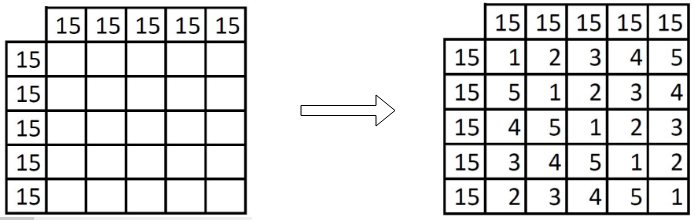
\includegraphics[width=\columnwidth]{example_kakuro.png}
  		\caption{Example of solving a 5x5 kakuro gird}
		\label{fig:example_kakuro}
    	 \end{center}
\end{figure}

\section{Implementation}
The following diagram reperesents the class diagrams of our project\\

\begin{figure}[h!]
    	 \begin{center}
		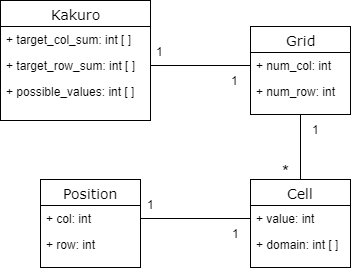
\includegraphics[width=\columnwidth]{class_diagram.png}
  		\caption{Class diagram}
		\label{fig:class_diagram}
    	 \end{center}
\end{figure}
The initial grid of the kakuro will be present in a file, which will contain the possible values of a cell and the target sum of each column and row. So for the grid in the figure \ref{fig:example_kakuro} we will have the following file\\
\begin{figure}[h!]
    	 \begin{center}
		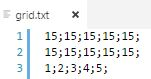
\includegraphics[width=3cm]{file_input.JPG}
  		\caption{File input}
		\label{fig:file_input}
    	 \end{center}
\end{figure}

\section{Solving - Forward Checking}
\begin{algorithm}
	\caption{Forward checking}
	\label{forward_checking}
	\begin{algorithmic}[1]
		\Procedure{ForwardChecking}{}
		\If {no free variable}
			\State return true
		\EndIf
		\State choose a free variable var
		\For {each value $v$ in $var.domain$}
			\State assign value to var
			\State update the domains of the free variable
			\If {no domain is empty or inconsistent}
				\If {ForwardChecking()}
					\State return true
				\EndIf
			\EndIf
		\EndFor
		\State return false
		\EndProcedure
	\end{algorithmic}
\end{algorithm}
\section{Monte Carlo Kakuro}

\section{Experimentals - Simulation}
    \begin{table}[!hbt]
        \begin{center}
        \caption{Simulation Parameters}
        \label{tab:simParameters}
        \begin{tabular}{|c|c|}
            \hline
           3x3 grid & $0.3$ s \\
            \hline
           5x5 grid & $0.3$ s \\
            \hline
           10x10 grid & $0.3$ s \\
            \hline
        \end{tabular}
        \end{center}
    \end{table}


\begin{thebibliography}{5}
    \bibitem{MonteCarloKakuro} 
    T.~Cazenave. {\em Monte-Carlo Kakuro}
\end{thebibliography}

\end{document}